\chapter{Анализ проблематики \dots}
\label{chapter1}

Это обзорно-аналитическая глава, в которой требуется отразить:

\begin{itemize}
	\item результат изучения различных существующих методов решения задач в рамках проблематики УИРа/диплома (иногда даже в смежных областях), это обзорный аспект, который пишется, в основном, на основе имеющейся литературы или/и программного обеспечения;
	\item сравнение (с какой-либо определенной целью) этих методов и средств.
\end{itemize}


%Большие отсупы --- это хорошо. Облегчает чтение длинных <<простыней>> текста
\section{Обзор методов геолокации по изобрадениям}

\begin{annotation}
В случае РСПЗ, так оформляется аннотация к разделу. Такая же аннотация, только более общая, должна быть для главы. После аннотации может следовать рабочая или финальная версия текста соответствующего раздела. В случае ПЗ, таких аннотаций быть не должно.
\end{annotation}

Задача определения места съемки фотографии довольно непроста из-за неоднозначности и недостаточности информации, содержащейся в одном изображении. Например, типичная пляжная сцена (море, солнце, песок, небо...) может быть заснята почти в любой точке земли. Даже достопремечательности не всегда могут служить абсолютными ориентирами: Эйфелева башня может указывать на Париж с Елисейскими полями, а может на Лас-Вегас или на село Париж в Челябинской области. В отсутствие подобных ориентиров люди полагаются на такие признаки как язык дорожных знаков, разметку, окружающую флору; опираясь на знания о внешнем мире для уточнения оценки местоположения. Традиционные системы компьютерного зрения часто не обладают подобными сведениями, полагаясь лишь на то что модно почерпнуть из тестовой выборки.

Результаты анализа полезно оформлять в виде таблиц (см. табл. \ref{tbl:cmp-1}).

\begin{table}%
\caption{Результаты сравнения нескольких программных систем}\label{tbl:cmp-1}
\centering
\begin{tabular}{|l|l|c|c|c|c|}

\hline

\textnumero & Название системы & Показатель 1 & Показатель 2 & Показатель 3 & Показатель 4 \\

\hline

\end{tabular}
\end{table}


\section{Изучение и сравнительный анализ алгоритмов глубокого обучения с целью выбора подхода к задаче}

Сначала приведем пример более сложной таблицы (см. табл. \ref{tbl:cmp-adv} и 
\ref{tbl:cmp-2}).

\begin{table}%
\caption{Таблица с длинным, многострочным названием, чтобы показать, как форматируется такой заголовок}
\label{tbl:cmp-adv}
\centering
\begin{tabular}{|l|l|c|c|c|c|}

\hline

\textnumero & Название системы & Показатель 1 & Показатель 2 & Показатель 3 & Показатель 4 \\

\hline

\end{tabular}
\label{tbl:cmp-2}
\end{table}


А теперь, продемонстрируем, как должна выглядеть иллюстрация (см. рис. \ref{pic:lambda-cube}).

\begin{figure}%
\begin{center}
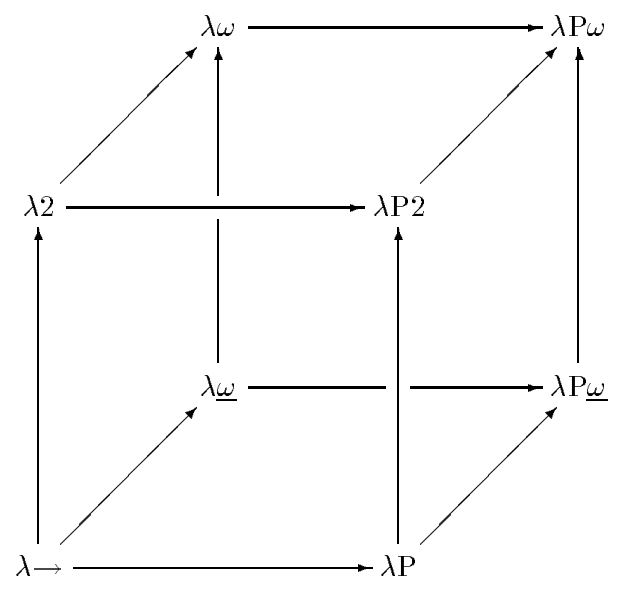
\includegraphics[width=.5\columnwidth]{./img/lambda-cube.png}%
\end{center}
\caption{Ламбда-куб Барендрегта}%
\label{pic:lambda-cube}%
\end{figure}

\dots





\section{Анализ алгоритмов пространственного разбиения поверхности земли для решения задачи классификации }

\dots





\section{Существующие решения задачи геолокации по изображениям}

\dots



\section{Анализ возможностей применения подхода transfer learning к проблеме геолокации с помощью глубокого обучения}


\section{Выводы}

Тут пишем выводы по результатам анализа: что и с какой целью было проанализировано, какие выводы из этого сделаны, как они повлияли (должны повлиять) на дальнейший ход работы. Результаты анализа приводятся попунктно, основные вывода из проделанного анализа. Например:

\begin{enumerate}
	\item Выполнен сравнительный анализ таких-то формальных систем с точки зрения применимости к решению такой-то задачи. Ни одна из проанализированных напрямую не подходит, поэтому требуется разработать вариацию на основе системы такой-то.
	\item Были проанализированы варианты программных архитектур на основе систем. С учетом требований к поддержке больших объемов данных и высоких требований к потенциалу модернизируемости, была выбрана за основу такая-то архитектура.
	\item Сравнительный анализ таких-то библиотек показал, что библиотека X проще в использовании, но менее производительна, в то время как библиотека Y обеспечивает высокую производительность, но и требует значительных трудозатрат для использования. В связи с такими-то соображениями были принято решение использовать такую-то библиотеку.
\end{enumerate}



\section{Постановка задачи дипломной работы/курсового проекта}

Это всегда последний пункт. Далее пишется постановка задачи, на основе выданного задания. Это должен быть связный текст в объеме до 1-1,5 страниц. В этом разделе необходимо раскрыть цели и задачи УИРа/диплома. 

